\subsection{Protobuf for Schema Definitions}\label{sec:protobuf_schema}
%TODO (Lucas): finish precise proofs 
Every document has a predefined schema which is agreed upon by all network participants. The Protobuf\footnote{\url{https://developers.google.com/protocol-buffers/}} message format is used for defining the document schema. It was chosen as a schema and serialization standard for its efficient binary format, broad support in different programming languages and fixed schema. An example of such a message is shown below in Fig. \ref{fig:example_document}. 

\begin{figure}[ht]
  \caption{An example protobuf definition}
  \label{fig:example_document}
  \begin{lstlisting}
  message ExampleDocument {
    string name = 1;
    repeated int numbers = 2;
  }\end{lstlisting}
\end{figure}

All documents that are supported by Centrifuge protocol are hosted on GitHub in a repository at \url{https://github.com/centrifuge/centrifuge-protobufs}.  

%TODO: write how CoreDocument has an include any.Any{} and that this is how the type is defined and add it as a field. mention that this structure was chosen because of a tradeoff in protobufs


\subsection{Precise proofs: Merkle tree format}\label{sec:precise_proofs}
Merkle trees are efficient ways to prove membership in a set. By encoding the leaves of the tree, a Merkle tree can be used to make a proof about the value of a field specific in the schema. The value of the field is prefixed with a byte encoded field path, $P$, and a salt, $S$. 


\subsubsection{Path encoding}
The reference for the path encoding is the precise-proofs\footnote{\url{https://github.com/centrifuge/precise-proofs}} library but is briefly summarized here. Protobuf uses 32bit unsigned integers to identify fields within a message uniquely. The property $p$ is defined using these values. The encoding of property names also supports nested messages, mappings, as well as repeated fields (arrays). 
\begin{equation}
    p_{F} = \mathsf{FieldToProperty}(F_{\texttt{name}})
\end{equation}

\begin{figure}[ht]
  \centering
  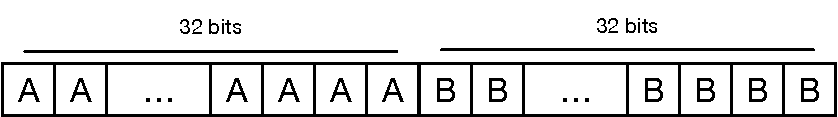
\includegraphics[width=11cm]{img/property_bits.pdf}
  \caption{The field numbers for a path \texttt{"A.B"} are concatenated into a fixed length delimited byte value} 
  \label{img:property_bits}
\end{figure}

In this paper, we refer to the fields by their human readable name using JavaScript-style dot notation for easier readability. However, the byte format will be used when encoding a leaves.


\subsubsection{Salts}
When proving, the hash of the sibling of the field is revealed. A salt is therefore added to the value of the leaves in order to avoid a rainbow table attack on sibling leaves revealed in a proof. The salt $F_{\mathsf{salt}}$ is stored in a special field on the \textit{CoreDocument} protobuf message called \texttt{salt} in form of a map where a salt is stored for each field by the property $p_F$.

\subsubsection{Construction of the tree}
For each leaf, $\lambda$, the name $P$, the salt $S$ and the value $v$ are appended and then hashed with $\mathtt{sha256}$.

\begin{eqnarray}
\lambda = \mathtt{sha256}(p_{F} \parallel F_{\texttt{value}} \parallel	 F_{\texttt{salt}})\\
\mathrm{T}(\mathrm{D}) = \mathcal{M}({\lambda_{1} \parallel \lambda_{2} \parallel ... \parallel \lambda_{n}})
\end{eqnarray}

\subsubsection{Merkle Proof Validation}\label{sec:merkle_proof_validation}
A Merkle proof can be seen as a function which proves if a provided field $P_\mathtt{field}$ is part of document. By calling the NFT mint method the value of these fields is revealed to the public. 
\begin{equation}
\begin{split}
v = \mathcal{M}_{\texttt{proof}}(A_{\texttt{anchor-current}},P_\mathtt{field},P_\mathtt{sibling-hashes}) \\
v \in \{0;1\}
\end{split}
\end{equation}
The $P_\mathtt{field}$  could be any field of the core document $d_C$ or the schema field $d_S$. The required $P_\mathtt{sibling-hashes}$ can be generated with the precise proofs library inside the node and contains the siblings of the field in each layer of the Merkle tree.  